\documentclass[ignorenonframetext,]{beamer}
\setbeamertemplate{caption}[numbered]
\setbeamertemplate{caption label separator}{: }
\setbeamercolor{caption name}{fg=normal text.fg}
\beamertemplatenavigationsymbolsempty
\usepackage{lmodern}
\usepackage{amssymb,amsmath}
\usepackage{ifxetex,ifluatex}
\usepackage{fixltx2e} % provides \textsubscript
\ifnum 0\ifxetex 1\fi\ifluatex 1\fi=0 % if pdftex
  \usepackage[T1]{fontenc}
  \usepackage[utf8]{inputenc}
\else % if luatex or xelatex
  \ifxetex
    \usepackage{mathspec}
  \else
    \usepackage{fontspec}
  \fi
  \defaultfontfeatures{Ligatures=TeX,Scale=MatchLowercase}
\fi
% use upquote if available, for straight quotes in verbatim environments
\IfFileExists{upquote.sty}{\usepackage{upquote}}{}
% use microtype if available
\IfFileExists{microtype.sty}{%
\usepackage{microtype}
\UseMicrotypeSet[protrusion]{basicmath} % disable protrusion for tt fonts
}{}
\newif\ifbibliography
\hypersetup{
            pdftitle={Tema 1 - Trabajando con R},
            pdfauthor={Juan Gabriel Gomila \& María Santos},
            pdfborder={0 0 0},
            breaklinks=true}
\urlstyle{same}  % don't use monospace font for urls
\usepackage{color}
\usepackage{fancyvrb}
\newcommand{\VerbBar}{|}
\newcommand{\VERB}{\Verb[commandchars=\\\{\}]}
\DefineVerbatimEnvironment{Highlighting}{Verbatim}{commandchars=\\\{\}}
% Add ',fontsize=\small' for more characters per line
\usepackage{framed}
\definecolor{shadecolor}{RGB}{248,248,248}
\newenvironment{Shaded}{\begin{snugshade}}{\end{snugshade}}
\newcommand{\KeywordTok}[1]{\textcolor[rgb]{0.13,0.29,0.53}{\textbf{#1}}}
\newcommand{\DataTypeTok}[1]{\textcolor[rgb]{0.13,0.29,0.53}{#1}}
\newcommand{\DecValTok}[1]{\textcolor[rgb]{0.00,0.00,0.81}{#1}}
\newcommand{\BaseNTok}[1]{\textcolor[rgb]{0.00,0.00,0.81}{#1}}
\newcommand{\FloatTok}[1]{\textcolor[rgb]{0.00,0.00,0.81}{#1}}
\newcommand{\ConstantTok}[1]{\textcolor[rgb]{0.00,0.00,0.00}{#1}}
\newcommand{\CharTok}[1]{\textcolor[rgb]{0.31,0.60,0.02}{#1}}
\newcommand{\SpecialCharTok}[1]{\textcolor[rgb]{0.00,0.00,0.00}{#1}}
\newcommand{\StringTok}[1]{\textcolor[rgb]{0.31,0.60,0.02}{#1}}
\newcommand{\VerbatimStringTok}[1]{\textcolor[rgb]{0.31,0.60,0.02}{#1}}
\newcommand{\SpecialStringTok}[1]{\textcolor[rgb]{0.31,0.60,0.02}{#1}}
\newcommand{\ImportTok}[1]{#1}
\newcommand{\CommentTok}[1]{\textcolor[rgb]{0.56,0.35,0.01}{\textit{#1}}}
\newcommand{\DocumentationTok}[1]{\textcolor[rgb]{0.56,0.35,0.01}{\textbf{\textit{#1}}}}
\newcommand{\AnnotationTok}[1]{\textcolor[rgb]{0.56,0.35,0.01}{\textbf{\textit{#1}}}}
\newcommand{\CommentVarTok}[1]{\textcolor[rgb]{0.56,0.35,0.01}{\textbf{\textit{#1}}}}
\newcommand{\OtherTok}[1]{\textcolor[rgb]{0.56,0.35,0.01}{#1}}
\newcommand{\FunctionTok}[1]{\textcolor[rgb]{0.00,0.00,0.00}{#1}}
\newcommand{\VariableTok}[1]{\textcolor[rgb]{0.00,0.00,0.00}{#1}}
\newcommand{\ControlFlowTok}[1]{\textcolor[rgb]{0.13,0.29,0.53}{\textbf{#1}}}
\newcommand{\OperatorTok}[1]{\textcolor[rgb]{0.81,0.36,0.00}{\textbf{#1}}}
\newcommand{\BuiltInTok}[1]{#1}
\newcommand{\ExtensionTok}[1]{#1}
\newcommand{\PreprocessorTok}[1]{\textcolor[rgb]{0.56,0.35,0.01}{\textit{#1}}}
\newcommand{\AttributeTok}[1]{\textcolor[rgb]{0.77,0.63,0.00}{#1}}
\newcommand{\RegionMarkerTok}[1]{#1}
\newcommand{\InformationTok}[1]{\textcolor[rgb]{0.56,0.35,0.01}{\textbf{\textit{#1}}}}
\newcommand{\WarningTok}[1]{\textcolor[rgb]{0.56,0.35,0.01}{\textbf{\textit{#1}}}}
\newcommand{\AlertTok}[1]{\textcolor[rgb]{0.94,0.16,0.16}{#1}}
\newcommand{\ErrorTok}[1]{\textcolor[rgb]{0.64,0.00,0.00}{\textbf{#1}}}
\newcommand{\NormalTok}[1]{#1}
\usepackage{longtable,booktabs}
\usepackage{caption}
% These lines are needed to make table captions work with longtable:
\makeatletter
\def\fnum@table{\tablename~\thetable}
\makeatother
\usepackage{graphicx,grffile}
\makeatletter
\def\maxwidth{\ifdim\Gin@nat@width>\linewidth\linewidth\else\Gin@nat@width\fi}
\def\maxheight{\ifdim\Gin@nat@height>\textheight0.8\textheight\else\Gin@nat@height\fi}
\makeatother
% Scale images if necessary, so that they will not overflow the page
% margins by default, and it is still possible to overwrite the defaults
% using explicit options in \includegraphics[width, height, ...]{}
\setkeys{Gin}{width=\maxwidth,height=\maxheight,keepaspectratio}

% Prevent slide breaks in the middle of a paragraph:
\widowpenalties 1 10000
\raggedbottom

\AtBeginPart{
  \let\insertpartnumber\relax
  \let\partname\relax
  \frame{\partpage}
}
\AtBeginSection{
  \ifbibliography
  \else
    \let\insertsectionnumber\relax
    \let\sectionname\relax
    \frame{\sectionpage}
  \fi
}
\AtBeginSubsection{
  \let\insertsubsectionnumber\relax
  \let\subsectionname\relax
  \frame{\subsectionpage}
}

\setlength{\parindent}{0pt}
\setlength{\parskip}{6pt plus 2pt minus 1pt}
\setlength{\emergencystretch}{3em}  % prevent overfull lines
\providecommand{\tightlist}{%
  \setlength{\itemsep}{0pt}\setlength{\parskip}{0pt}}
\setcounter{secnumdepth}{0}

\title{Tema 1 - Trabajando con R}
\author{Juan Gabriel Gomila \& María Santos}
\date{}

\begin{document}
\frame{\titlepage}

\section{Conociendo R}\label{conociendo-r}

\begin{frame}{¿Qué es R?}

\begin{figure}
\centering
\includegraphics{Imgs/RLogo.jpg}
\caption{}
\end{figure}

\begin{itemize}
\tightlist
\item
  Entorno de programación para el análisis estadístico y gráfico de
  datos
\item
  Software libre
\item
  Sintaxis sencilla e intuitiva
\item
  Enorme comunidad de usuarios (Comprehensive R Archive Network, CRAN)
\item
  ¿Aún tenéis dudas de por qué usarlo?
  \href{https://www.r-bloggers.com/why-use-r-five-reasons/}{Haz click
  aquí}
\end{itemize}

\end{frame}

\begin{frame}{¿Qué es RStudio?}

En este curso usaremos RStudio como interfaz gráfica de usuario de R
para todos los sistemas operativos

Es un entorno integrado para utilizar y programar con R

\begin{figure}
\centering
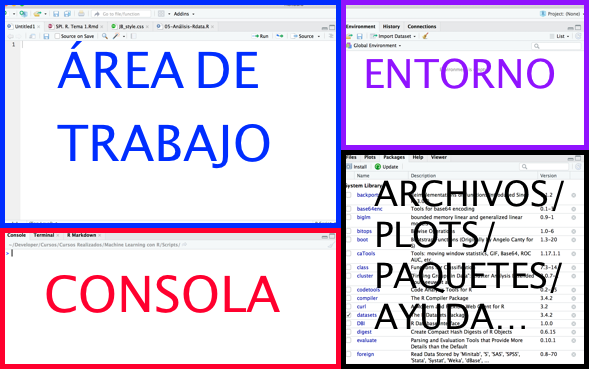
\includegraphics{Imgs/InterfazRStudio.png}
\caption{}
\end{figure}

\end{frame}

\begin{frame}[fragile]{Cómo instalar R}

\textbf{Si sois de Windows o Mac}

\begin{enumerate}
\def\labelenumi{\arabic{enumi}.}
\tightlist
\item
  Id a \href{http://cran.r-project.org/}{CRAN}
\item
  Pulsad sobre el enlace correspondiente a vuestro sistema operativo
\item
  Seguid las instrucciones de instalación correspondientes
\end{enumerate}

\textbf{Si trabajáis con Ubuntu o Debian}

\begin{enumerate}
\def\labelenumi{\arabic{enumi}.}
\tightlist
\item
  Abrid la terminal, estando conectados a internet
\item
  Introducid lo siguiente: \texttt{sudo\ aptitude\ install\ r-base}
\end{enumerate}

\end{frame}

\begin{frame}[fragile]{Cómo instalar RStudio}

\begin{enumerate}
\def\labelenumi{\arabic{enumi}.}
\tightlist
\item
  \href{http://www.rstudio.com/products/rstudio/download/}{Obtener
  RStudio}
\item
  \textbf{Solo si utilizáis Linux}, ejecutad en una terminal la
  siguiente instrucción para completar la instalación:
  \texttt{sudo\ dpkg\ -i\ rstudio-\textless{}version\textgreater{}-i386.deb},
  donde \texttt{version} refiere a la versión concreta que se haya
  descargado
\end{enumerate}

\begin{figure}
\centering

\includegraphics{Imgs/RSLogo.jpg}
\caption{}
\end{figure}

\end{frame}

\begin{frame}{Trabajando con RStudio}


\includegraphics{Imgs/Disquete.png} 
\includegraphics{Imgs/Carpeta.png}

\includegraphics{Imgs/RScript.png} 
\includegraphics{Imgs/RNotebook.png}

\includegraphics{Imgs/RMarkdown.png} 
\includegraphics{Imgs/Shiny.png}

\includegraphics{Imgs/TextFile.png} 
\includegraphics{Imgs/C++File.png}

\includegraphics{Imgs/RSweave.png} 
\includegraphics{Imgs/RHTML.png}

\includegraphics{Imgs/RPresentation.png}

\includegraphics{Imgs/RDocumentation.png}

\begin{figure}
\centering
\includegraphics{Imgs/Easy.jpg}
\caption{}
\end{figure}

\end{frame}

\begin{frame}[fragile]{Cómo pedir ayuda}

\begin{itemize}
\tightlist
\item
  \texttt{help()}: obtener ayuda por consola
\item
  \texttt{??...}: obtener ayuda por consola
\item
  Pestaña \texttt{Help} de Rstudio
\item
  \href{https://www.rstudio.com/wp-content/uploads/2015/02/rmarkdown-cheatsheet.pdf}{Cheat
  Sheet de RStudio}
\item
  Buscar en San Google (stackoverflow, R project\ldots{})
\item
  Foro del curso
\end{itemize}

\begin{figure}
\centering

\includegraphics{Imgs/help.png}
\caption{}
\end{figure}

\end{frame}

\begin{frame}[fragile]{Paquetes: cómo instalarlos y cargarlos}

Paquete. Librería con funciones y datos que no necesariamente vienen
instaladas de serie

\begin{itemize}
\tightlist
\item
  \texttt{install.packages("nombre\_paquete",\ dep\ =\ TRUE)}: instala o
  actualiza un paquete de R
\item
  \texttt{library(nombre\_del\_paquete)}: carga un paquete ya instalado
\end{itemize}

\end{frame}

\section{Utilizando R como
calculadora}\label{utilizando-r-como-calculadora}

\begin{frame}[fragile]{Calculadora básica - Operaciones}

\begin{longtable}[]{@{}ll@{}}
\toprule
Código & Operación\tabularnewline
\midrule
\endhead
\texttt{+} & Suma\tabularnewline
\texttt{-} & Resta\tabularnewline
\texttt{*} & Multiplicación\tabularnewline
\texttt{/} & División\tabularnewline
\texttt{\^{}} & Potencia\tabularnewline
\texttt{\%/\%} & Cociente entero\tabularnewline
\texttt{\%\%} & Resto de división entera\tabularnewline
\bottomrule
\end{longtable}

\end{frame}

\begin{frame}[fragile]{Calculadora básica - Operaciones}

\begin{longtable}[]{@{}ll@{}}
\toprule
Código & Significado\tabularnewline
\midrule
\endhead
\texttt{pi} &
\href{https://es.wikipedia.org/wiki/Número_π}{\(\pi\)}\tabularnewline
\texttt{Inf} &
\href{https://es.wikipedia.org/wiki/Infinito}{\(\infty\)}\tabularnewline
\texttt{NaN} & Indeterminación (Not a Number)\tabularnewline
\texttt{NA} & Valor desconocido (Not Available)\tabularnewline
\bottomrule
\end{longtable}

\end{frame}

\begin{frame}[fragile]{Calculadora básica - Operaciones}

\begin{Shaded}
\begin{Highlighting}[]
\DecValTok{2}\OperatorTok{+}\DecValTok{2}
\end{Highlighting}
\end{Shaded}

\begin{verbatim}
[1] 4
\end{verbatim}

\begin{Shaded}
\begin{Highlighting}[]
\DecValTok{77}\OperatorTok\DecValTok{5}
\end{Highlighting}
\end{Shaded}

\begin{verbatim}
[1] 15
\end{verbatim}

\begin{Shaded}
\begin{Highlighting}[]
\DecValTok{77}\OperatorTok\DecValTok{5}
\end{Highlighting}
\end{Shaded}

\begin{verbatim}
[1] 2
\end{verbatim}

\end{frame}

\begin{frame}[fragile]{Calculadora básica - Funciones}

\begin{longtable}[]{@{}ll@{}}
\toprule
Código & Función\tabularnewline
\midrule
\endhead
\texttt{sqrt(x)} & \(\sqrt{x}\)\tabularnewline
\texttt{exp(x)} & \(e^x\)\tabularnewline
\texttt{log(x)} & \(\ln(x)\)\tabularnewline
\texttt{log10(x)} & \(\log_{10}(x)\)\tabularnewline
\texttt{log(x,a)} & \(\log_a(x)\)\tabularnewline
\texttt{abs(x)} & \(\begin{vmatrix}x\end{vmatrix}\)\tabularnewline
\bottomrule
\end{longtable}

\end{frame}

\begin{frame}[fragile]{Calculadora básica - Funciones}

\begin{Shaded}
\begin{Highlighting}[]
\KeywordTok{sqrt}\NormalTok{(}\DecValTok{9}\NormalTok{)}
\end{Highlighting}
\end{Shaded}

\begin{verbatim}
[1] 3
\end{verbatim}

\begin{Shaded}
\begin{Highlighting}[]
\KeywordTok{log}\NormalTok{(}\KeywordTok{exp}\NormalTok{(}\DecValTok{1}\NormalTok{))}
\end{Highlighting}
\end{Shaded}

\begin{verbatim}
[1] 1
\end{verbatim}

\begin{Shaded}
\begin{Highlighting}[]
\KeywordTok{log}\NormalTok{(}\DecValTok{1000}\NormalTok{,}\DecValTok{10}\NormalTok{)}
\end{Highlighting}
\end{Shaded}

\begin{verbatim}
[1] 3
\end{verbatim}

\begin{Shaded}
\begin{Highlighting}[]
\KeywordTok{log10}\NormalTok{(}\DecValTok{1000}\NormalTok{)}
\end{Highlighting}
\end{Shaded}

\begin{verbatim}
[1] 3
\end{verbatim}

\end{frame}

\begin{frame}[fragile]{Calculadora básica - Combinatoria}

\begin{longtable}[]{@{}ll@{}}
\toprule
Código & Operación\tabularnewline
\midrule
\endhead
\texttt{factorial(x)} &
\href{https://es.wikipedia.org/wiki/Factorial}{\(x!\)}\tabularnewline
\texttt{choose(n,m)} &
\(\begin{pmatrix}n\\ m\end{pmatrix}\)\tabularnewline
\bottomrule
\end{longtable}

\vspace{0.2cm}

\begin{itemize}
\tightlist
\item
  Número factorial. Se define como número factorial de un número entero
  positivo \(n\) como \(n!=n\cdot(n-1)\cdots 2\cdot 1\)
\item
  \href{https://es.wikipedia.org/wiki/Coeficiente_binomial}{Coeficiente
  binomial}. Se define el coeficiente binomial de \(n\) sobre \(m\) como
  \[\begin{pmatrix}n\\ m\end{pmatrix}=\frac{n!}{m!(n-m)!}\]
\end{itemize}

\end{frame}

\begin{frame}{Calculadora básica - Combinatoria}

\href{https://es.wikipedia.org/wiki/Triángulo_de_Pascal}{Triángulo de
Pascal}. \usepackage{mathdots} \usepackage{yhmath} \usepackage{mathdots}
\usepackage{MnSymbol} \[\begin{matrix}
&&&&&1&&&&&\\
&&&&1&&1&&&&\\
&&&1&&2&&1&&&\\
&&1&&3&&3&&1&&\\
&1&&4&&6&&4&&1&\\
1&&5&&10&&10&&5&&1\end{matrix}\]

que se corresponde con \ldots{}

\end{frame}

\begin{frame}{Calculadora básica - Combinatoria}

\[\begin{matrix}
&&&&\begin{pmatrix}0\\0\end{pmatrix}&&&&\\
&&&\begin{pmatrix}1\\0\end{pmatrix}&&\begin{pmatrix}1\\1\end{pmatrix}&&&\\
&&\begin{pmatrix}2\\0\end{pmatrix}&&\begin{pmatrix}2\\1\end{pmatrix}&&\begin{pmatrix}2\\2\end{pmatrix}&&\\
&\begin{pmatrix}3\\0\end{pmatrix}&&\begin{pmatrix}3\\1\end{pmatrix}&&\begin{pmatrix}3\\2\end{pmatrix}&&\begin{pmatrix}3\\3\end{pmatrix}&\\
\begin{pmatrix}4\\0\end{pmatrix}&&\begin{pmatrix}4\\1\end{pmatrix}&&\begin{pmatrix}4\\2\end{pmatrix}&&\begin{pmatrix}4\\3\end{pmatrix}&&\begin{pmatrix}4\\4\end{pmatrix}\end{matrix}\]

\end{frame}

\begin{frame}[fragile]{Calculadora básica - Combinatoria}

\begin{Shaded}
\begin{Highlighting}[]
\KeywordTok{factorial}\NormalTok{(}\DecValTok{5}\NormalTok{)}
\end{Highlighting}
\end{Shaded}

\begin{verbatim}
[1] 120
\end{verbatim}

\begin{Shaded}
\begin{Highlighting}[]
\KeywordTok{choose}\NormalTok{(}\DecValTok{4}\NormalTok{,}\DecValTok{2}\NormalTok{)}
\end{Highlighting}
\end{Shaded}

\begin{verbatim}
[1] 6
\end{verbatim}

\begin{Shaded}
\begin{Highlighting}[]
\KeywordTok{factorial}\NormalTok{(}\DecValTok{6}\NormalTok{)}
\end{Highlighting}
\end{Shaded}

\begin{verbatim}
[1] 720
\end{verbatim}

\begin{Shaded}
\begin{Highlighting}[]
\KeywordTok{factorial}\NormalTok{(}\DecValTok{5}\NormalTok{)}\OperatorTok{*}\DecValTok{6}
\end{Highlighting}
\end{Shaded}

\begin{verbatim}
[1] 720
\end{verbatim}

\end{frame}

\begin{frame}[fragile]{Trigonometría en radianes}

\begin{longtable}[]{@{}ll@{}}
\toprule
Código & Función\tabularnewline
\midrule
\endhead
\texttt{sin(x)} & \(\sin(x)\)\tabularnewline
\texttt{cos(x)} & \(\cos(x)\)\tabularnewline
\texttt{tan(x)} & \(\tan(x)\)\tabularnewline
\texttt{asin(x)} & \(\arcsin(x)\)\tabularnewline
\texttt{acos(x)} & \(\arccos(x)\)\tabularnewline
\texttt{atan(x)} & \(\arctan(x)\)\tabularnewline
\bottomrule
\end{longtable}

\end{frame}

\begin{frame}[fragile]{Trigonometría en radianes}

\begin{Shaded}
\begin{Highlighting}[]
\KeywordTok{sin}\NormalTok{(pi}\OperatorTok{/}\DecValTok{2}\NormalTok{)}
\end{Highlighting}
\end{Shaded}

\begin{verbatim}
[1] 1
\end{verbatim}

\begin{Shaded}
\begin{Highlighting}[]
\KeywordTok{cos}\NormalTok{(pi)}
\end{Highlighting}
\end{Shaded}

\begin{verbatim}
[1] -1
\end{verbatim}

\begin{Shaded}
\begin{Highlighting}[]
\KeywordTok{tan}\NormalTok{(}\DecValTok{0}\NormalTok{)}
\end{Highlighting}
\end{Shaded}

\begin{verbatim}
[1] 0
\end{verbatim}

\end{frame}

\begin{frame}{Trigonometría en radianes}

\begin{figure}
\centering
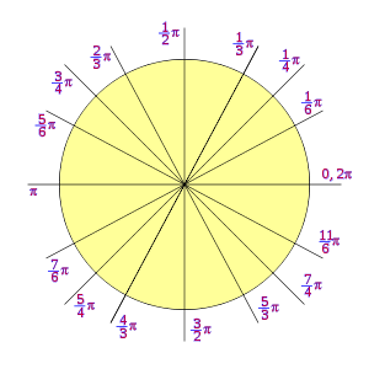
\includegraphics{Imgs/trigon.png}
\caption{Circunferencia Goniométrica}
\end{figure}

\end{frame}

\begin{frame}[fragile]{Un pequeño adelanto}

\begin{Shaded}
\begin{Highlighting}[]
\NormalTok{x =}\StringTok{ }\KeywordTok{seq}\NormalTok{(}\DecValTok{0}\NormalTok{,}\DecValTok{2}\OperatorTok{*}\NormalTok{pi,}\FloatTok{0.1}\NormalTok{)}
\KeywordTok{plot}\NormalTok{(x,}\KeywordTok{sin}\NormalTok{(x),}\DataTypeTok{type=}\StringTok{"l"}\NormalTok{,}\DataTypeTok{col=}\StringTok{"blue"}\NormalTok{,}\DataTypeTok{lwd=}\DecValTok{3}\NormalTok{, }\DataTypeTok{xlab=}\KeywordTok{expression}\NormalTok{(x), }\DataTypeTok{ylab=}\StringTok{""}\NormalTok{)}
\KeywordTok{lines}\NormalTok{(x,}\KeywordTok{cos}\NormalTok{(x),}\DataTypeTok{col=}\StringTok{"green"}\NormalTok{,}\DataTypeTok{lwd=}\DecValTok{3}\NormalTok{)}
\KeywordTok{lines}\NormalTok{(x, }\KeywordTok{tan}\NormalTok{(x), }\DataTypeTok{col=}\StringTok{"purple"}\NormalTok{,}\DataTypeTok{lwd=}\DecValTok{3}\NormalTok{)}
\KeywordTok{legend}\NormalTok{(}\StringTok{"bottomleft"}\NormalTok{,}\DataTypeTok{col=}\KeywordTok{c}\NormalTok{(}\StringTok{"blue"}\NormalTok{,}\StringTok{"green"}\NormalTok{,}\StringTok{"purple"}\NormalTok{),}
     \DataTypeTok{legend=}\KeywordTok{c}\NormalTok{(}\StringTok{"Seno"}\NormalTok{,}\StringTok{"Coseno"}\NormalTok{, }\StringTok{"Tangente"}\NormalTok{), }\DataTypeTok{lwd=}\DecValTok{3}\NormalTok{, }\DataTypeTok{bty=}\StringTok{"l"}\NormalTok{)}
\end{Highlighting}
\end{Shaded}

\begin{center}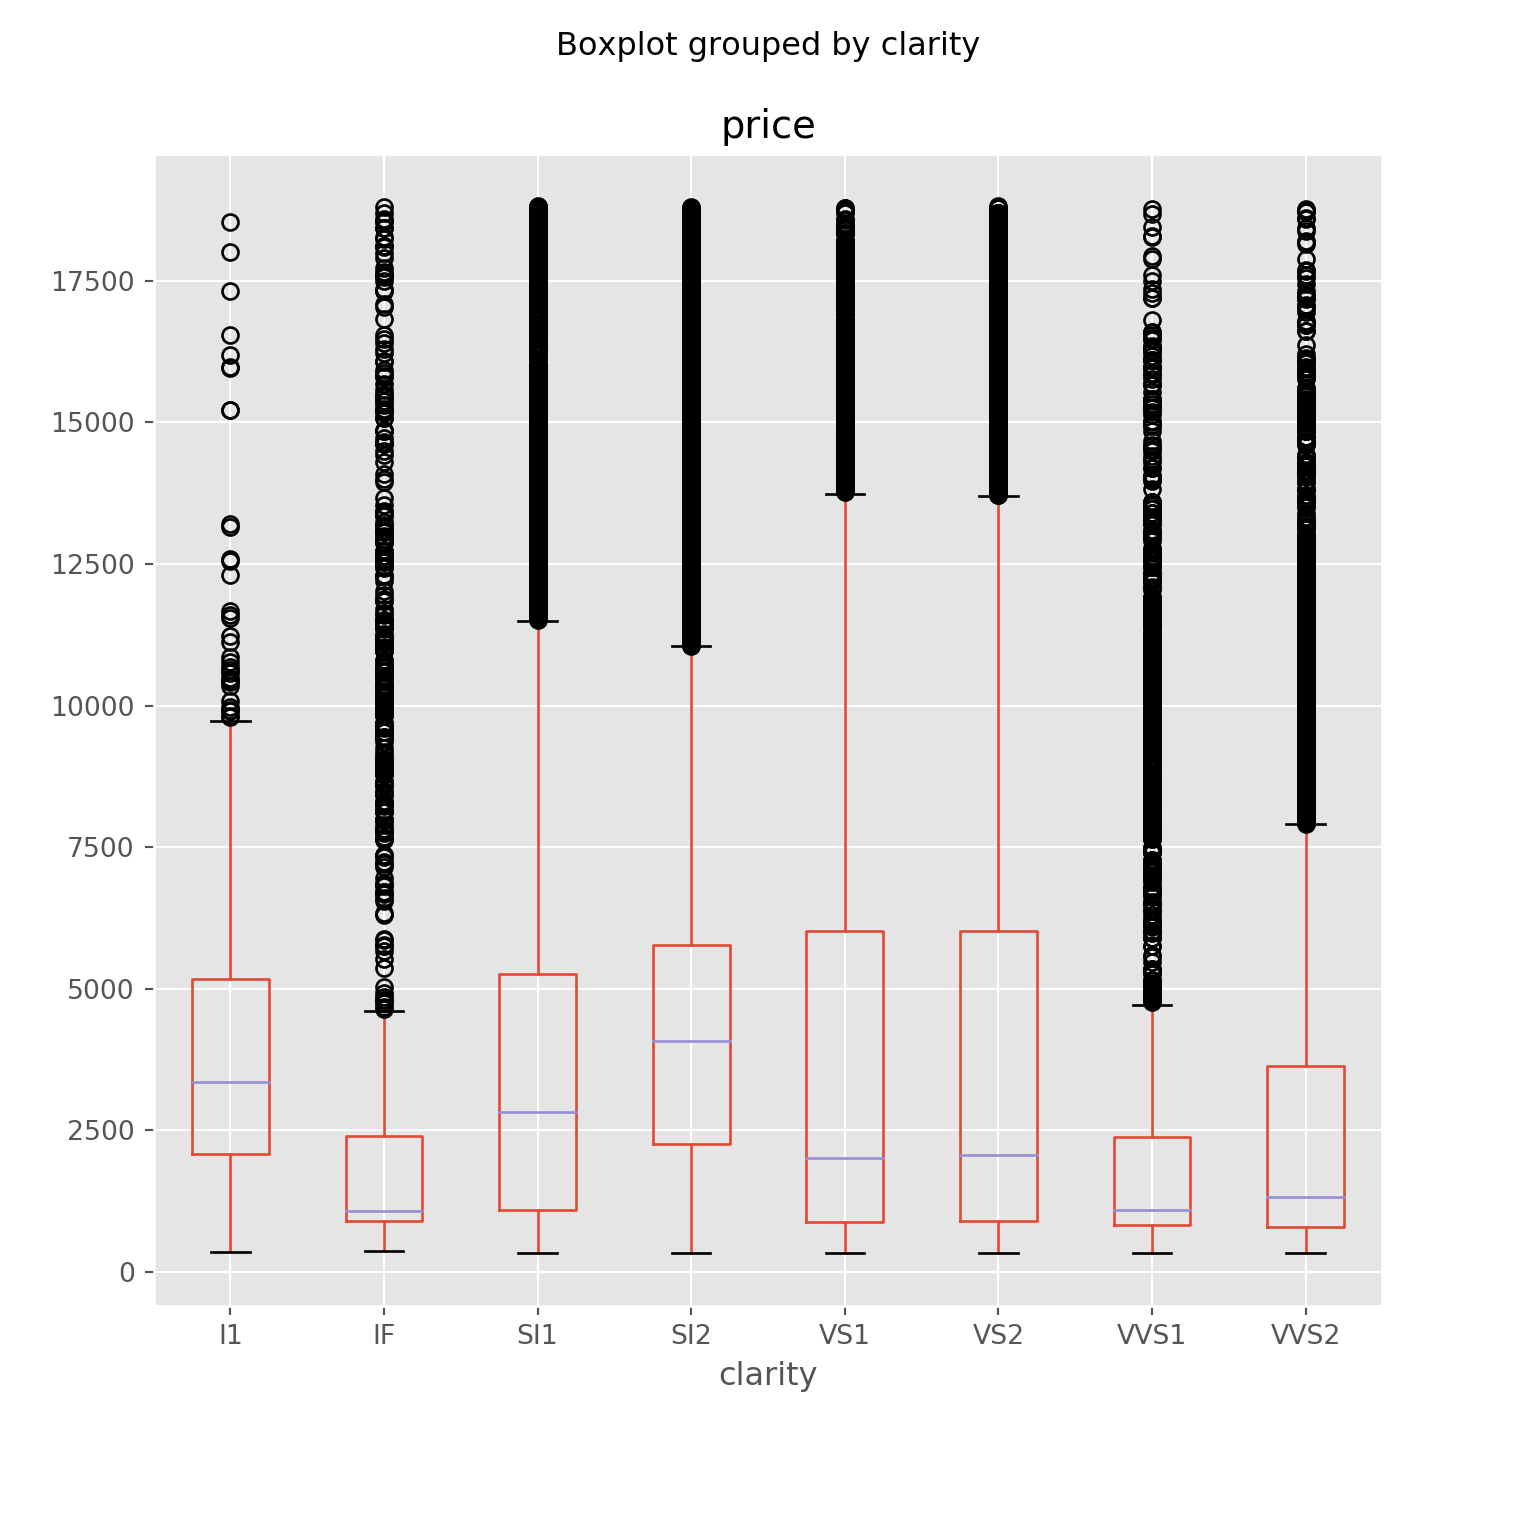
\includegraphics{Tema1_files/figure-beamer/unnamed-chunk-5-1} \end{center}

\end{frame}

\begin{frame}[fragile]{Números en coma flotante}

\begin{longtable}[]{@{}ll@{}}
\toprule
\begin{minipage}[b]{0.10\columnwidth}\raggedright\strut
Código\strut
\end{minipage} & \begin{minipage}[b]{0.27\columnwidth}\raggedright\strut
Función\strut
\end{minipage}\tabularnewline
\midrule
\endhead
\begin{minipage}[t]{0.10\columnwidth}\raggedright\strut
\texttt{print(x,n)}\strut
\end{minipage} & \begin{minipage}[t]{0.27\columnwidth}\raggedright\strut
Muestra las \(n\) cifras significativa del número \(x\)\strut
\end{minipage}\tabularnewline
\begin{minipage}[t]{0.10\columnwidth}\raggedright\strut
\texttt{round(x,n)}\strut
\end{minipage} & \begin{minipage}[t]{0.27\columnwidth}\raggedright\strut
Redondea a \(n\) cifras significativas un resultado o vector numérico
\(x\)\strut
\end{minipage}\tabularnewline
\begin{minipage}[t]{0.10\columnwidth}\raggedright\strut
\texttt{floor(x)}\strut
\end{minipage} & \begin{minipage}[t]{0.27\columnwidth}\raggedright\strut
\(\lfloor x\rfloor\), parte entera por defecto de \(x\)\strut
\end{minipage}\tabularnewline
\begin{minipage}[t]{0.10\columnwidth}\raggedright\strut
\texttt{ceiling(x)}\strut
\end{minipage} & \begin{minipage}[t]{0.27\columnwidth}\raggedright\strut
\(\lceil x\rceil\), parte entera por exceso de \(x\)\strut
\end{minipage}\tabularnewline
\begin{minipage}[t]{0.10\columnwidth}\raggedright\strut
\texttt{trunc(x)}\strut
\end{minipage} & \begin{minipage}[t]{0.27\columnwidth}\raggedright\strut
Parte entera de \(x\), eliminando la parte decimal\strut
\end{minipage}\tabularnewline
\bottomrule
\end{longtable}

\end{frame}

\begin{frame}[fragile]{Números en coma flotante}

\begin{Shaded}
\begin{Highlighting}[]
\KeywordTok{print}\NormalTok{(pi,}\DecValTok{5}\NormalTok{)}
\end{Highlighting}
\end{Shaded}

\begin{verbatim}
[1] 3.1416
\end{verbatim}

\begin{Shaded}
\begin{Highlighting}[]
\KeywordTok{round}\NormalTok{(pi,}\DecValTok{5}\NormalTok{)}
\end{Highlighting}
\end{Shaded}

\begin{verbatim}
[1] 3.14159
\end{verbatim}

\begin{Shaded}
\begin{Highlighting}[]
\KeywordTok{floor}\NormalTok{(pi)}
\end{Highlighting}
\end{Shaded}

\begin{verbatim}
[1] 3
\end{verbatim}

\begin{Shaded}
\begin{Highlighting}[]
\KeywordTok{ceiling}\NormalTok{(pi)}
\end{Highlighting}
\end{Shaded}

\begin{verbatim}
[1] 4
\end{verbatim}

\end{frame}

\begin{frame}[fragile]{Variables y funciones}

\begin{itemize}
\tightlist
\item
  \texttt{nombre\_variable\ =\ valor}: define una variable con dicho
  valor
\item
  \texttt{nombre\_función\ =\ function(variable)\{función\}}: define una
  función
\end{itemize}

\begin{Shaded}
\begin{Highlighting}[]
\NormalTok{miVariable =}\StringTok{ }\DecValTok{4}
\NormalTok{doble =}\StringTok{ }\ControlFlowTok{function}\NormalTok{(x)\{}\DecValTok{2}\OperatorTok{*}\NormalTok{x\}}
\KeywordTok{doble}\NormalTok{(miVariable)}
\end{Highlighting}
\end{Shaded}

\begin{verbatim}
[1] 8
\end{verbatim}

\begin{Shaded}
\begin{Highlighting}[]
\NormalTok{cuadrado =}\StringTok{ }\ControlFlowTok{function}\NormalTok{(x)\{x}\OperatorTok{^}\DecValTok{2}\NormalTok{\}}
\KeywordTok{cuadrado}\NormalTok{(miVariable)}
\end{Highlighting}
\end{Shaded}

\begin{verbatim}
[1] 16
\end{verbatim}

\end{frame}

\begin{frame}[fragile]{Números complejos}

\begin{longtable}[]{@{}ll@{}}
\toprule
Código & Función\tabularnewline
\midrule
\endhead
\texttt{a+bi} &
\href{https://es.wikipedia.org/wiki/Número_complejo}{Número
complejo}\tabularnewline
\texttt{complex(real=...,imaginary=...)} & Número complejo en forma
binómica\tabularnewline
\texttt{complex(modulus=...,argument=...)} & Número complejo en forma
polar\tabularnewline
\bottomrule
\end{longtable}

\end{frame}

\begin{frame}[fragile]{Números complejos}

\begin{longtable}[]{@{}ll@{}}
\toprule
Código & Función\tabularnewline
\midrule
\endhead
\texttt{sqrt(as.complex(-x))} & \(\sqrt{-x}\)\tabularnewline
\texttt{Re(x)} & Parte real de \(x\)\tabularnewline
\texttt{Im(x)} & Parte imaginaria de \(x\)\tabularnewline
\texttt{Mod(x)} & Módulo de \(x\)\tabularnewline
\texttt{Arg(x)} & Argumento de \(x\)\tabularnewline
\texttt{Conj(x)} & Conjugado de \(x\)\tabularnewline
\bottomrule
\end{longtable}

\end{frame}

\begin{frame}[fragile]{Números complejos}

\begin{Shaded}
\begin{Highlighting}[]
\NormalTok{z =}\StringTok{ }\DecValTok{2}\OperatorTok{+}\NormalTok{3i}
\NormalTok{z2 =}\StringTok{ }\KeywordTok{complex}\NormalTok{(}\DataTypeTok{real =} \DecValTok{2}\NormalTok{, }\DataTypeTok{imaginary =} \OperatorTok{-}\DecValTok{3}\NormalTok{)}
\KeywordTok{Re}\NormalTok{(z)}
\end{Highlighting}
\end{Shaded}

\begin{verbatim}
[1] 2
\end{verbatim}

\begin{Shaded}
\begin{Highlighting}[]
\KeywordTok{Im}\NormalTok{(z)}
\end{Highlighting}
\end{Shaded}

\begin{verbatim}
[1] 3
\end{verbatim}

\begin{Shaded}
\begin{Highlighting}[]
\KeywordTok{Conj}\NormalTok{(z2)}
\end{Highlighting}
\end{Shaded}

\begin{verbatim}
[1] 2+3i
\end{verbatim}

\end{frame}

\begin{frame}{Números complejos}

\begin{figure}
\centering
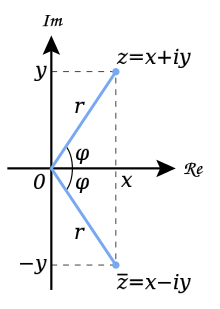
\includegraphics{Imgs/complex.png}
\caption{}
\end{figure}

\end{frame}

\end{document}
